\documentclass{article}
\usepackage{tikz}
\usetikzlibrary{decorations.markings, calc}

% Custom line style with parameterized midpoint label
\tikzset{
  line via circle/.style args={#1}{
    postaction={
      decoration={
        markings,
        mark=at position 0.5 with {
          \node[circle, draw, fill=white, inner sep=2pt, font=\footnotesize] {#1};
        }
      },
      decorate
    }
  }
}

\begin{document}

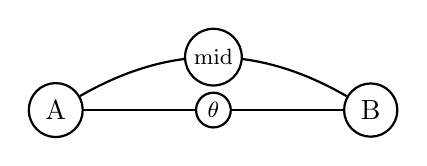
\begin{tikzpicture}[node distance=4cm, thick]
  % Define two nodes
  \node[draw, circle] (A) {A};
  \node[draw, circle, right of=A] (B) {B};

  % Use custom style with label parameter
  \draw[line via circle={$\theta$}] (A) -- (B);
  \draw[line via circle={mid}] (A) to[bend left] (B);
\end{tikzpicture}

\end{document}